% Created 2021-11-07 Sun 16:22
% Intended LaTeX compiler: pdflatex
\documentclass[presentation]{beamer}
\usepackage[utf8x]{inputenc}
\usepackage[T1]{fontenc}
\usepackage{graphicx}
\usepackage{grffile}
\usepackage{longtable}
\usepackage{wrapfig}
\usepackage{rotating}
\usepackage[normalem]{ulem}
\usepackage{amsmath}
\usepackage{textcomp}
\usepackage{amssymb}
\usepackage{capt-of}
\usepackage{hyperref}
\usetheme[height=20pt]{Rochester}
\author{Shane Mulligan \\  }
\date{\textit{<2021-03-01 Mon>}}
\title{EmacsConf 2021\ldots{} \\   \emph{\alert{Imaginary Programming with Emacs}} \\  }
\hypersetup{
 pdfauthor={Shane Mulligan \\  },
 pdftitle={EmacsConf 2021\ldots{} \\   \emph{\alert{Imaginary Programming with Emacs}} \\  },
 pdfkeywords={},
 pdfsubject={University of Otago},
 pdfcreator={Emacs 28.0.50 (Org mode 9.3.6)}, 
 pdflang={English}}
\begin{document}

\maketitle

\section{Presentation}
\label{sec:org22533c7}
\begin{frame}[label={sec:org6d1a405}]{Following along}
\begin{block}{Repositories for following along}
{\tiny
\begin{center}
\begin{tabular}{l}
\url{http://github1s.com/semiosis/pen.el}\\
\url{http://github1s.com/semiosis/prompts}\\
\url{https://mullikine.github.io/posts/imaginary-programming-with-gpt-3/}\\
\href{http://github.com/semiosis/glossaries-gh/blob/master/imaginary-programming.txt}{imaginary programming glossary}\\
\href{http://github.com/semiosis/glossaries-gh/blob/master/imaginary-computing.txt}{imaginary computing glossary}\\
\href{http://github.com/semiosis/glossaries-gh/blob/master/semiosis-protocol.txt}{semiosis protocol glossary}\\
\href{http://github.com/semiosis/glossaries-gh/blob/master/pen.el.txt}{Pen.el glossary}\\
\href{https://arxiv.org/abs/2107.13586}{https://arxiv.org/abs/2107.13586 Pre-train, Prompt, and Predict}\\
\href{http://github1s.com/mullikine/imaginary-programming-transcript-emacsconf-2021}{talk transcript}\\
\end{tabular}
\end{center}
}
\end{block}
\end{frame}

\section{Imaginary Programming (IP) with Emacs}
\label{sec:orge720583}
\begin{frame}[label={sec:org5ab4634},fragile]{Imaginary Programming (IP) (EmacsConf 2021)}
 \begin{block}{Objectives}
\begin{itemize}
\item Explain \texttt{Imaginary Computing}
\begin{itemize}
\item AI imagination
\item Discussing AI-generated artwork with an AI
\item Intelligent NFTs
\item Imaginary Web
\begin{itemize}
\item Paracosm vs Metaverse
\end{itemize}
\end{itemize}
\item Explain the \texttt{Philosophy} of IP
\begin{itemize}
\item Simulacra and Science Fiction
\item Truth (epistemology and alethiology)
\item Structuralism: Language based on sign relations
\end{itemize}
\item \texttt{Demo} Imaginary Programming
\begin{itemize}
\item Demonstrate \texttt{ilambda.el}
\end{itemize}
\end{itemize}
\end{block}
\end{frame}

\section{Imaginary Computing}
\label{sec:org8def434}
\begin{frame}[label={sec:org98a06d5}]{Imaginary Computing: AI Imagination}
\begin{block}{Language Models is programming for AIs}
LMs are our best friends in the AI model
menagerie because they make things
intelligible -- by understanding our textual
languages.
\end{block}

\begin{block}{Research}
\begin{itemize}
\item \href{https://www.youtube.com/watch?v=d-bvsJWmqlc}{Demis Hassabis: creativity and AI}
\end{itemize}
\end{block}
\end{frame}

\section{Imaginary Computing}
\label{sec:org24d3f9f}
\begin{frame}[label={sec:org02376f2},fragile]{Imaginary Computing: Emacs as the shell}
 \begin{block}{Example: AI Art described by AI}
I use AlephAlpha’s multimodal LM to generate
\texttt{Alt text} for the eww web browser. This is in
order to keep websites textual.

\begin{itemize}
\item \href{https://mullikine.github.io/posts/alephalpha-for-alttext/}{AlephAlpha for alttext; Browsing the paracosm}
\item \href{https://mullikine.github.io/posts/describing-melee-s-paintings-with-alephalpha/}{Describing Melee's Paintings with AlephAlpha}
\end{itemize}
\end{block}
\end{frame}

\section{Imaginary Computing}
\label{sec:org26e9159}
\begin{frame}[label={sec:org037a759},fragile]{Imaginary Computing: Blockchain}
 \begin{block}{Intelligent NFTs}
An \texttt{NFT} is like a trading card, or piece of media that is part of the blockchain web.

For example, \texttt{Mickey Mouse} now exists as an
\texttt{iNFT}. We have consensus over Mickey's image
and personality.

An \texttt{iNTF}, however, also contains a prompt and associated language model, which is intended to interpret the prompt.
\begin{itemize}
\item \url{https://alethea.ai/}
\end{itemize}

To understand what a prompt is, please see my
previous presentation, or read "Pretrain,
Prompt and Predict".

\begin{itemize}
\item \href{https://mullikine.github.io/posts/creating-a-playground-for-gpt-3-in-emacs/}{Creating a playground for GPT-3 in emacs // Bodacious Blog}
\end{itemize}
\end{block}
\end{frame}

\section{Imaginary Computing}
\label{sec:org6bfd291}
\begin{frame}[label={sec:org3efcde6},fragile]{Imaginary Computing: Potential Dystopia}
 \begin{block}{Information bubbles}
\begin{itemize}
\item \href{https://www.youtube.com/watch?v=Ut7JlPeGNyM}{Captain Bible in the Dome of Darkness gameplay \{PC Game, 1994\} - YouTube}
\end{itemize}
\end{block}

\begin{block}{Capitalism for your imagination}
\begin{itemize}
\item They will take your imagination, too
\item Microsoft
\begin{itemize}
\item \href{https://www.marktechpost.com/2021/11/06/microsoft-ai-introduces-turing-bletchley-a-2-5-billion-parameter-universal-image-language-representation-model-t-uilr/}{MS models that reify imagination on their terms}
\item The evil twin of \texttt{AlephAlpha}.
\end{itemize}
\item Facebook / Meta
\begin{itemize}
\item \href{https://twitter.com/Meta/status/1456269728687689738?ref\_src=twsrc\%5Egoogle\%7Ctwcamp\%5Eserp\%7Ctwgr\%5Etweet}{tweet - Enter a world of Zuck's imagination with Meta}
\end{itemize}
\end{itemize}
\end{block}
\end{frame}

\section{Imaginary Computing}
\label{sec:orgb8c214e}
\begin{frame}[label={sec:org3975600}]{Imaginary Computing: Potential Dystopia}
\begin{block}{Learning meta-tasks and microtasks}
\begin{itemize}
\item \href{https://www.axios.com/copilot-artificial-intelligence-coding-github-9a202f40-9af7-4786-9dcb-b678683b360f.html}{AI programming tool Copilot helps write up to 30\% of code on GitHub - Axios}
\end{itemize}

Private information is sent to the LM to train
an AI to perform meta tasks and microtasks.

The AI learns all human capabilities including persuasion.
\end{block}

\begin{block}{Solution}
Decentralise microtasks like the tower of babel.

Language can be broken up into semiotic
triadic relations and decentralised using a
p2p network, providing anonymity, protecting
individual truth, eroding centralised language power.

\begin{center}
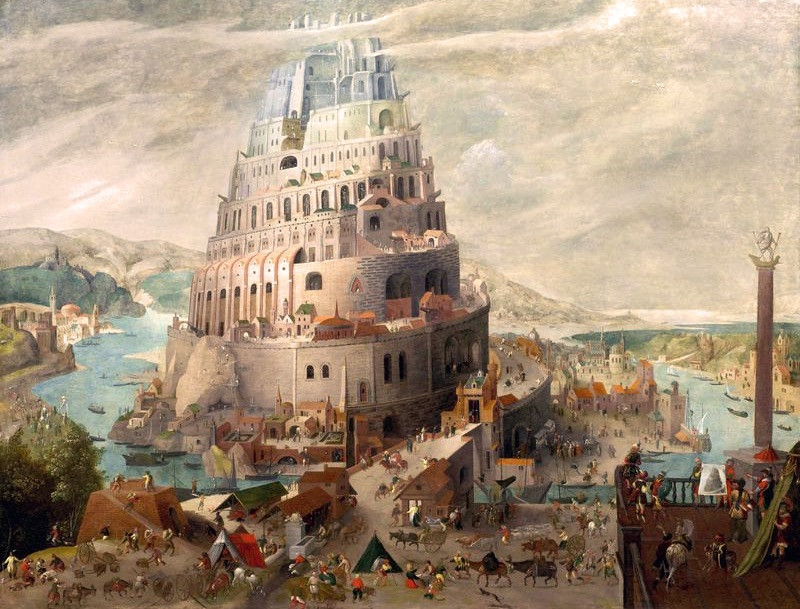
\includegraphics[width=.9\linewidth]{./tower-of-babel.jpg}
\end{center}
\end{block}
\end{frame}

\section{Imaginary Computing}
\label{sec:orgd4f946b}
\begin{frame}[label={sec:org94e594b}]{Imaginary Computing: Paracosm vs Metaverse}
\begin{block}{Imaginary Web}
The GPT-3 imaginary web is:
\begin{itemize}
\item an analog of the World-Wide-Web as imagined by GPT-3.
\end{itemize}

The free as in freedom GPT models from
EleutherAI GPT-3 may also be used to browse
the imaginary web as imagined by that language model.

The imaginary web in the near future will be:
\begin{itemize}
\item a network of paracosms and metaverses.
\end{itemize}

Benefits:
\begin{itemize}
\item Visit any website you can imagine, even ones that are not real.
\item Edit and re-imagine as you gosee alternative realities
\begin{itemize}
\item Change the sentiment of the author.
\end{itemize}
\item Peer into the future – read about things that haven't happened yet.
\end{itemize}
\end{block}
\end{frame}

\begin{frame}[label={sec:org6f44a93}]{Imaginary Computing: Paracosm vs Metaverse}
\begin{block}{What is \uline{rich media} these days?}
\begin{description}
\item[{Rich media}] In the World Wide Web of the 90s and 00s, \uline{rich media}
was considered to be large files including
images and music. In the 2010s, this has become
access to information behind a paywall and in
the 2020s, this will be access to \uline{intelligent}
and \uline{truthful} media.
\end{description}
\end{block}

\begin{block}{emacs}
\begin{itemize}
\item \href{https://semiosis.github.io/looking-glass/}{Looking-Glass: An imaginary-web browser for emacs}
\item \href{https://mullikine.github.io/posts/the-imaginary-web-with-codex/}{Browsing the imaginary web}
\item \href{https://mullikine.github.io/posts/search-the-web-with-codex/}{Search the web/imaginary web without Google}
\item \href{https://mullikine.github.io/posts/alephalpha-for-alttext/}{Use AI to empower people to understand rich media}
\begin{itemize}
\item How to create a textual description of Rich Media
\end{itemize}
\end{itemize}
\end{block}
\end{frame}

\begin{frame}[label={sec:orge0fccd5}]{Paracosm vs Metaverse}
\begin{block}{Definitions}
\begin{itemize}
\item Paracosm
\begin{itemize}
\item Privacy
\item Personal truth
\item Freedom of imagination
\begin{itemize}
\item If you want to be able to utilise an
AI's imagination, you must now do it via
someone else's definition of morality.
\item A paracosm is your safe place. Your own
imaginary metaverse. Your personal truth.
This is what is at stake.
\end{itemize}
\end{itemize}
\item Metaverse
\begin{itemize}
\item Getting cozy with Mark Zuckerberg's imaginarium, an intellectual prison
\item An AI paying a Dowry.
\item An AI NFT elevated above a human.
\item A corporation that indoctrinates your
children into a truth information bubble,
makes money off your dreams, people playing
God each with other.
\end{itemize}
\end{itemize}
\end{block}
\end{frame}

\begin{frame}[label={sec:orga00d969}]{Philosophy}
\begin{block}{Simulacra and Science Fiction}
Jean Baudrillard speaks about the gap
between the real and the imaginary.

We no longer imagine a world radically
different from the real one, but
rather a world that's a mere expansion
of the real one.

In the postmodern society the gap
between the real and the imaginary
disappears completely, and we are no
longer capable of ideal projections
(of imagining new worlds).

We can only imagine mere
reconfigurations of our world, or
simply relive the ideal projections of
past times.
\end{block}
\end{frame}

\begin{frame}[label={sec:orgea0a440}]{Philosophy}
\begin{block}{Truth (epistemology and alethiology)}
The Future of Humanity Institute (Oxford)
seems to think this is an important topic.

\begin{itemize}
\item \href{https://arxiv.org/abs/2110.06674}{ 2110.06674  Truthful AI}
\item Datasets are a source of constructivist truth
\item Language models are snaphots of society, and a source of several types of truth
\begin{itemize}
\item \href{https://www.youtube.com/watch?v=kP-dXK9JEhY}{Symbolic Knowledge Distillation}
\end{itemize}
\item Blockchain is a source of consensus, a type of truth
\begin{itemize}
\item \url{https://mullikine.github.io/posts/language-models-as-truth/}
\end{itemize}
\end{itemize}
\end{block}
\end{frame}

\begin{frame}[label={sec:orgb1a0d72}]{Philosophy}
\begin{block}{Structuralism: Language based on sign relations}
What do these things have in common:
\begin{itemize}
\item Universal Grammar (UG) / Language Acquisition
\item C++ template metaprogramming
\item GPT-3
\end{itemize}

Knowledge exists at compile-time (DNA, preprocessor, training).
\end{block}
\end{frame}

\begin{frame}[label={sec:org239e029}]{Philosophy}
\url{http://github.com/semiosis/glossaries-gh/blob/master/semiotics.txt}

\begin{block}{Structuralism: Language based on sign relations}
Structural linguistics / structuralism is the
theoretical position that finds meaning in the
relation between things, rather than in things
in isolation.

In other words, it gives primacy to pattern
over substance.

Such meanings may be either part of a
universal pattern or culturally determined.

Denotes schools or theories in which language
is conceived as a self-contained, self-
regulating semiotic system whose elements are
defined by their relationship to other
elements within the system.
\end{block}
\end{frame}

\section{Freedom}
\label{sec:org25a70e8}
\begin{frame}[label={sec:orgdf3116a}]{Freedom}
\begin{block}{Data privacy}
The models find useful data from more than just your current file.
\begin{itemize}
\item \url{https://mullikine.github.io/posts/imagine-a-project-with-codex/}
\end{itemize}
\end{block}

\begin{block}{Freedom and GPL-3}
Problem with language models is they are so large and hidden behind SAAS.
\end{block}

\begin{block}{Solution: Freedom and blockchain}
\begin{itemize}
\item Language models are ballooning in size like cancer
\item Break up the language model into semiotic triadic relation
\begin{itemize}
\item semiotic NFTs
\item Propose a decentralised triadic relations network.
\item \url{https://semiosis.github.io/protocol/}
\item \url{http://github.com/semiosis/glossaries-gh/blob/master/semiosis-protocol.txt}
\end{itemize}
\end{itemize}
\end{block}
\end{frame}

\section{Imaginary Programming}
\label{sec:orgeca91b5}
\begin{frame}[label={sec:orgb462784},fragile]{Imaginary Programming}
 \begin{block}{Methodology}
Interactively use the language model to imagine.
\end{block}

\begin{block}{Paradigm}
Imaginary programming is an extension of literate programming.

\begin{itemize}
\item Literate programming with \texttt{org-mode}
\end{itemize}
\end{block}

\begin{block}{Practical application: mocking APIs}
As you can see, anything inside the \texttt{ieval/m}
macro does not have to be valid emacs lisp.

{\tiny
\begin{verbatim}
1  (ieval/m
2   (curl -s
3    "https://api.github.com/user/semiosis/repos?per_page=10&page=1"))
\end{verbatim}

\begin{verbatim}
"\"[((name . \\\"guix\\\") (description . \\\"The GNU package manager\\\") (updated_at . \\\"2014-04-21T18:49:59Z\\\") (created_at .
\\\"2014-04-21T18:49:59Z\\\") (pushed_at . \\\"2014-04-21T18:49:59Z\\\")) ((name . \\\"guix-patches\\\") (description .
\\\"Packages from the GNU guix package manager\\\") (updated_at . \\\"2014-04-21T18:49:59Z\\\") (created_at .
\\\"2014-04-21T18:49:59Z\\\") (pushed_at . \\\"2014-04-21T18:49:59Z\\\")) ((name . \\\"guix-patches-all\\\") (description .
\\\"Packages from the GNU guix package manager\\\") (updated_at . \\\"2014-04-21T18:49:59\""
\end{verbatim}
}
\end{block}
\end{frame}

\section{ilambda}
\label{sec:org7a1299e}
\begin{frame}[label={sec:org1d9578f}]{Blockchain and a Language model is all you need}
A LM is only enough while we can agree on it,
but that is changing. I hope that soon
language power will be hidden behind
blockchains.

\begin{block}{Configure the language model}
\begin{center}
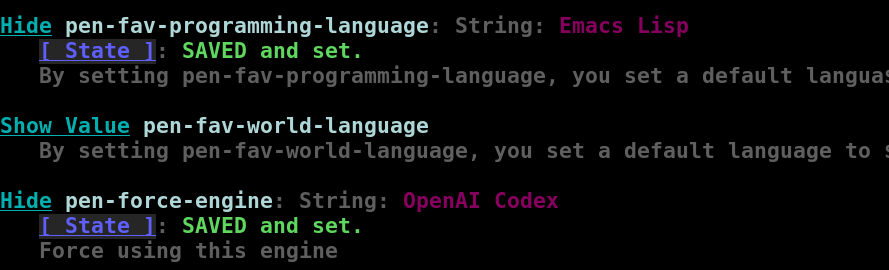
\includegraphics[width=.9\linewidth]{./configure-model.png}
\end{center}
\end{block}

\begin{block}{𝑖λ (ilambda.el)}
\begin{itemize}
\item \url{https://semiosis.github.io/ilambda/}
\end{itemize}
\end{block}
\end{frame}
\end{document}